
\section{System Analysis} \label{sec:analysis}

This section deals with the analysis of the aforementioned system of a wind turbine.
First, the description of the ODE system, which is insufficient for an implementation, is presented (\autoref{sec:analysis:ODE}) and the problems encountered are briefly described.

Second, the implementation of the system via transfer function is introduced \autoref{sec:analysis:tf}.
All important steps to implement the system in Matlab are shown.
By using figures published by Fragoso et al.– \cite{Fragoso_et_al_2017} the implementation in Matlab is verified.

The following chapter (\autoref{sec:condes}) is dealing with controller design. One important step of controller design is the relative gain array, which is conducted at the end of tis section.

\subsection{Simulation of ODE system} \label{sec:analysis:ODE}

Fragoso et al.~ \cite{Fragoso_et_al_2017} present a system of ODE for the wind turbine model.
As described in \autoref{sec:intro:model_eq} the model is subdivided into two parts.
The electrical subsystem is based in on two algebraic equations (\autoref{eq:intro:tau_em}, \autoref{eq:intro:P_g}).

For the mechanical part an ODE is given
\begin{align}
    J_t \frac{d \omega_t}{dt} = \tau_a - \tau_{em}, \label{eq:analysis:ODE_mechanical}
\end{align}
where $\tau_a$ is the aerodynamic torque and defined as
\begin{align}
    \tau_a = \frac{1}{2} \rho \pi R^3 \frac{C_p\left( \lambda, \beta\right)}{\lambda} v^2.
\end{align}
The power coefficient $C_p$ is only described by a figure (see Figure 4 in \cite{Fragoso_et_al_2017}).
In Fragosos work \cite[p. 54 ff.]{Fragoso_PhD_2016} a function for $C_p$ is derived and also a figure shows the global course of the function (see Figure 3.8, p. 56).
In this function nine heuristic parameters are used to determine the characteristics.
It is unclear if this function is also used in the work of Fragoso et al.~ or not.

In the appendix of Fragosos PhD-thesis there are tabulated value for $C_p$.
These were implemented as a lookuptable in Matlab.
By using the lookup table, values for $C_p$ could be determined, but the solutions of the ODE were not in a realistic range of values.

\begin{lstlisting}[style=Matlab-editor,caption={Matlab function for lookuptable. With this function we can get a corresponding $C_p$ value for given $\beta$ and $\lambda$. The \texttt{.csv}-file can be found in the GitHub repository under},captionpos=b,label={list:analysis:lookup}]
% Loading tabulated values as .csv file
p.lookup = readtable('lookuptable_c_p.csv');
% Setting corresponding column names 
p.lookup.Properties.VariableNames = {'wind_speed','rotor_speed','U','i_a','P_e','P_m','lambda','C_p','C_q','beta'};

% Looking up values for values of lambda and beta
function C_p = power_coefficient(lambda,beta,lookup)
    C_p = interp1(lookup.lambda(lookup.beta==beta),lookup.C_p(lookup.beta==beta),lambda);
end
\end{lstlisting}

Even if it is possible to get correct values for $C_p$, we still have only one ODE and a algebraic equation.
This is not representing a systems with two systems states.

Due to the problems mentioned here, the representation and solution of the system in state space was not pursued further and the transfer function mentioned in the Fragose et al.~ was used instead.

\subsection{Implementation of transfer function model} \label{sec:analysis:tf}

All controllers will be designed based on a linear model.
For different wind speeds $v$ Fragoso et al.~ identified five different linear models.
The pitch angel $\beta$ and the duty cycle $\alpha$ are the systems states.
The outputs are the rotational speed of the blade $\omega_r$ and the generated electric power $P_g$.
\begin{align}
    \begin{pmatrix}
        \omega_r \\
        P_g
      \end{pmatrix} = 
      G(s) 
      \begin{pmatrix}
        \beta \\
        \alpha
      \end{pmatrix} + G_D(s) v
\end{align}

The transferfunctions $G$ and $G_D$ where identified for windspeed $v=\left[6,7,8,9,10 \right] \si{\metre\per\second}$.
The results can be found in \cite[Table 2]{Fragoso_et_al_2017} and will not be reprinted here.

\begin{table}[H]
    \label{tab:analysis:import_var}
    \caption{Compilation of the most important variables, their meaning, unit and value range. The value ranges in italics are estimated values derived from figures. In addition, only the deviation $\Delta v$ is given, as we consider the disturbance in the following sections only as a deviation from zero. That is why we also consider a maximum value range between -1 and 1, as we would enter the \textit{domain} of another transfer function for larger values.}
    \centering
    \begin{tabular}{cllcc} \toprule
        Variable & Name & Interpration & Unit & Range \\ \midrule
        $\Delta v$ & change in windspeed & disturbance  & \si{\metre\per\second} & $\mathit{\left[-1,1\right]}$\\
        $\beta$ & pitch angle & state & \si{\degree}& $\left[0,25\right]$ \\
        $\alpha$ & duty cycle& state & 1 & $\left[0,1\right]$\\
        $\omega_r$ & rotational speed of blade & input & rpm & $\mathit{\left[1400,2000 \right]}$  \\
        $P_g$ &generated electric power &input & \si{\watt} &  $\mathit{\left[3,9 \right]}$\\ \bottomrule
    \end{tabular}
    \label{tab:analysis:constraints}
\end{table}

\subsubsection*{Implementation in Matlab}

To generate the transfer functions in Matlab the \texttt{tf}-command and the \texttt{table} function are used.

\begin{lstlisting}[style=Matlab-editor,caption={},captionpos=b,label={list:analysis:tf}]
% Wind speed: 6 m/s
G_S_num_6 = {-8.059,-405.4;-0.0081479,4.4195};
G_S_denom_6 = {[75.27,17.35,1],[28.25, 16.47, 1];[0, 16.873, 1],[0, 1.7589, 1]};
G_D_num_6 = {364.9; 1.139};
G_D_denom_6 = {[118.3, 21.76, 1];[65.28, 17.09, 1]};

... Wind speeds 7,8,9 an 10 m/s ...

% Making a table to store all transfer_function
varNames = ["wind_speed","G_S_numerator","G_S_denominator","G_D_numerator","G_D_denominator","G_S","G_D","RGA"];
table_tf = table;
% Naming the columns in the table
table_tf.Properties.VariableNames = varNames;

% Filling the table with numerator and denominator
table_tf(1,1:5) = {6,G_S_num_6,G_S_denom_6,G_D_num_6,G_D_denom_6};
...
table_tf(5,1:5) = {10,G_S_num_10,G_S_denom_10,G_D_num_10,G_D_denom_10};
table_tf.Properties.VariableNames = varNames(1:5);

% For loop for creating transfer function by using tf-command
for i = 1:5
    table_tf{i,6} = {tf(table_tf{i,"G_S_numerator"}{:},table_tf{i,"G_S_denominator"}{:})};
    table_tf{i,7} = {tf(table_tf{i,"G_D_numerator"}{:},table_tf{i,"G_D_denominator"}{:})};
    table_tf{i,8} = {NaN};
end
\end{lstlisting}

For each transfer function modeling the system behaviour for different wind speeds we have a numerator and denominator for the systems transfer function $G$ and the disturbance system $G_D$.
Those are stored as arrays \texttt{G\_num\_6}, \texttt{G\_D\_denom\_6}, etc.~, where the 6 at the end depicting the transfer function for a wind speed of $\SI{6}{\metre \per \second}$.

In line 17 ff. the numerator and denominator of all transfer function are stored in the table initialized in line 12.
Using the \texttt{tf}-command inside a \texttt{for-loop} (line 23 ff.) the transfer function is defined.
In line 14 every column of the table gets a name.

\subsubsection{Verifying the implementation}

The goal of verification is the recreation of relative step responses shown by Fragoso et al.~(\autoref{fig:analysis:fig_step_response}).
The figure is used as a benchmark.
If the global course of the step response can be readjusted, then one can assume that the model is implemented correctly.

\begin{figure}[H]
    \center
    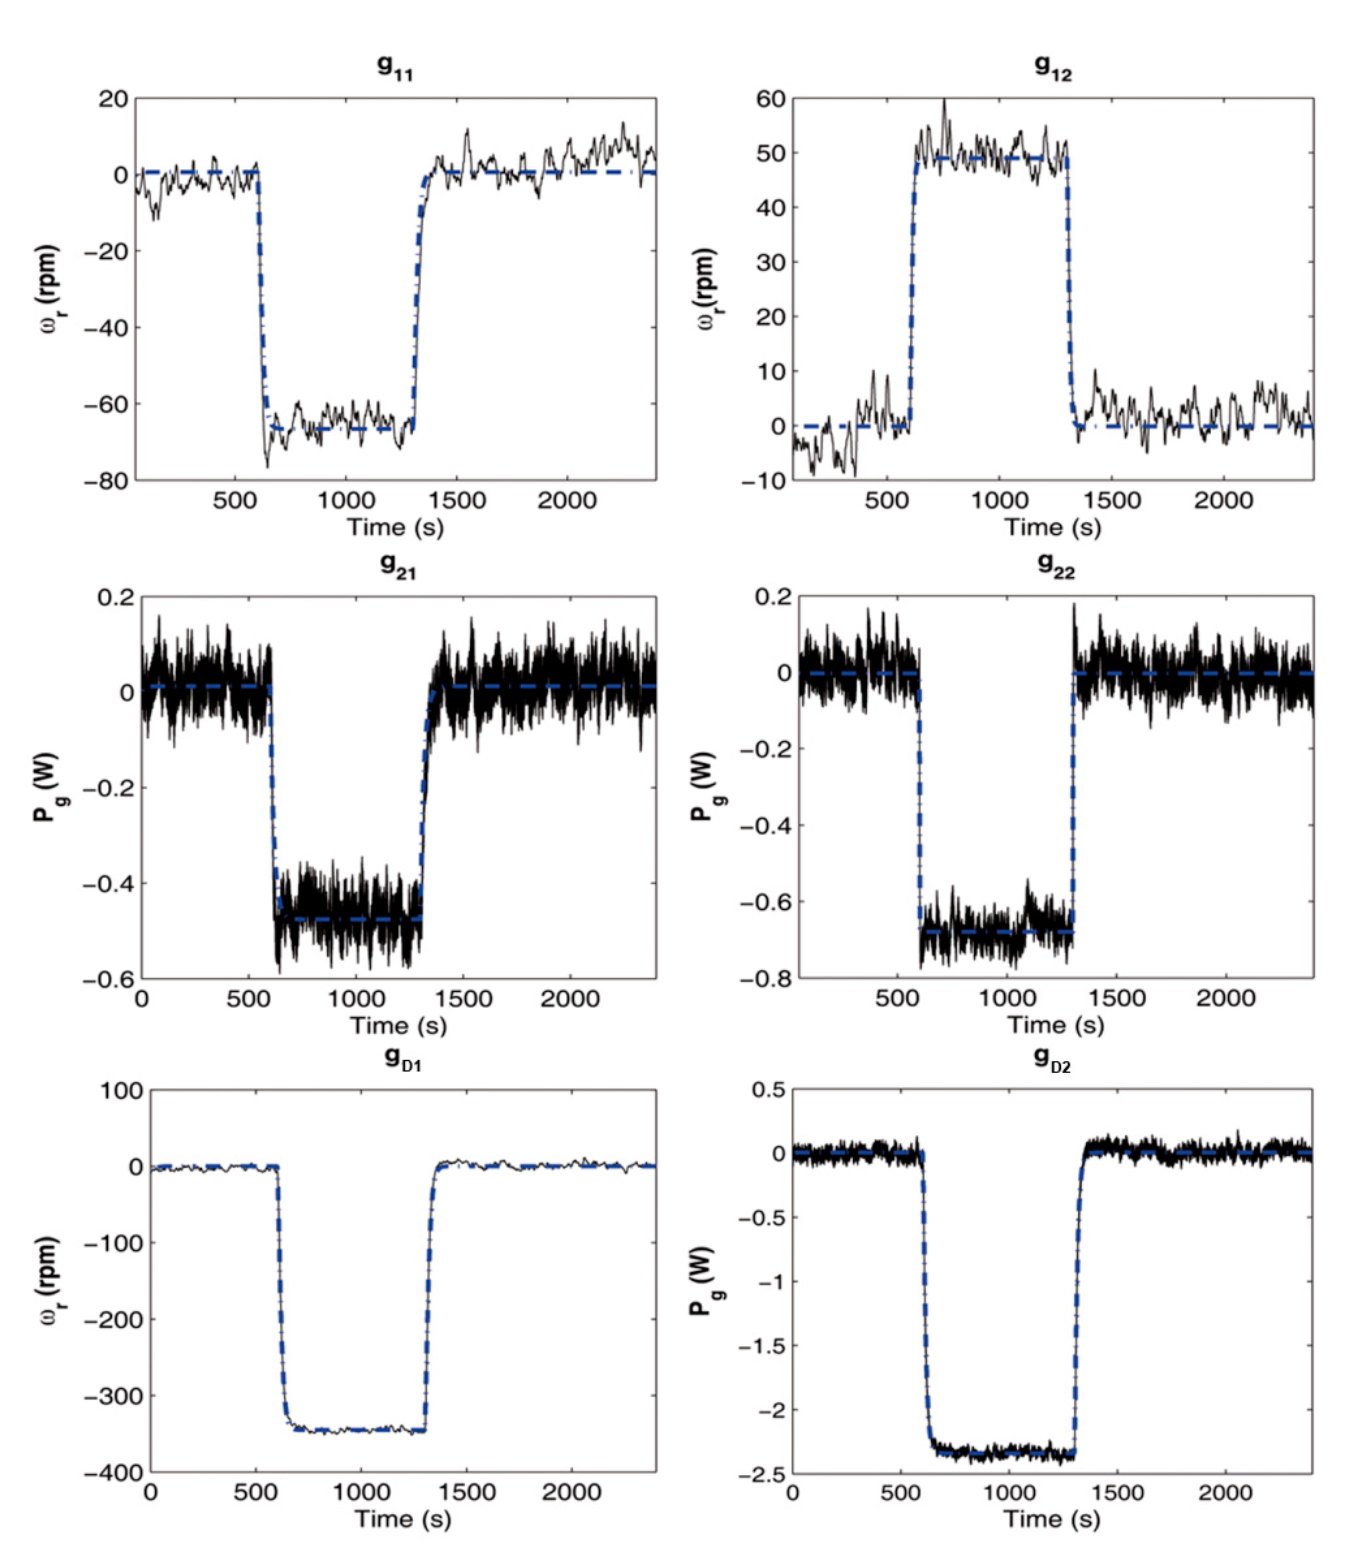
\includegraphics[scale=0.5]{fig/Fragoso_et_al_2017_fig6.png}
    \caption{The figure presented by \cite{Fragoso_et_al_2017} shows the relative step response of the identified system (dashed line) and the real system (solid) line.}
    \label{fig:analysis:fig_step_response}
\end{figure}

The six figures are labeled as $g_{ij}$ as changing input $i$ and showing the influence on output $j$.
The bottom two are referring to the influence of disturbance changes (changes in wind speed) when inputs are changed.
Unfortunately the exact values are not given in the paper and therefore must be reverse engineered.

\begin{table}[H]
    \caption{The tables shows the influence of an input to a single output. The table can be seen as an other way of displaying the results from \autoref{fig:analysis:fig_step_response}.}
    \centering
    \begin{tabular}{ccccc} \toprule
        Figure & Input & $\Delta$ & Output & $\Delta$ \\ \midrule
        $g_{11}$ & $\beta$    & \SI{7}{\degree}               & $\omega_r$  & $\SI{-70}{rpm}$ \\
        $g_{12}$ & $\alpha$   & $-0.1$                        & $\omega_r$  & $\SI{50}{rpm}$ \\
        $g_{21}$ & $\beta$    & \SI{12}{\degree}              & $P_g$       & $\SI{-0.5}{\watt}$ \\
        $g_{22}$ & $\alpha$   & $-0.1$                        & $P_g$       & $\SI{-0.7}{\watt}$ \\
        $g_{D1}$ & $v_{wind}$ & $\SI{-1}{\metre\per\second}$  & $\omega_r$  & $\SI{-300}{rpm}$ \\
        $g_{D2}$ & $v_{wind}$ & $\SI{-2}{\metre\per\second}$  & $P_g$       & $\SI{-2.3}{\watt}$ \\ \bottomrule
    \end{tabular}
    \label{tab:analysis:changes}
\end{table}

From left to right the first row of \autoref{tab:analysis:changes} can be read as: For figure $g_{11}$ the input $\beta$ is changed by \SI{7}{\degree} and will result in reducing the rotational speed $\omega_r$ by \SI{70}{rpm}.
All six figures presented by Fragaso et al.~ can be recreated by the values given in \autoref{tab:analysis:changes}.
\autoref{fig:analysis:recreate_step_changes} is one example representing the subfigure $g_{11}$ and using the values of the first row.

\begin{figure}[h!]
    \center
    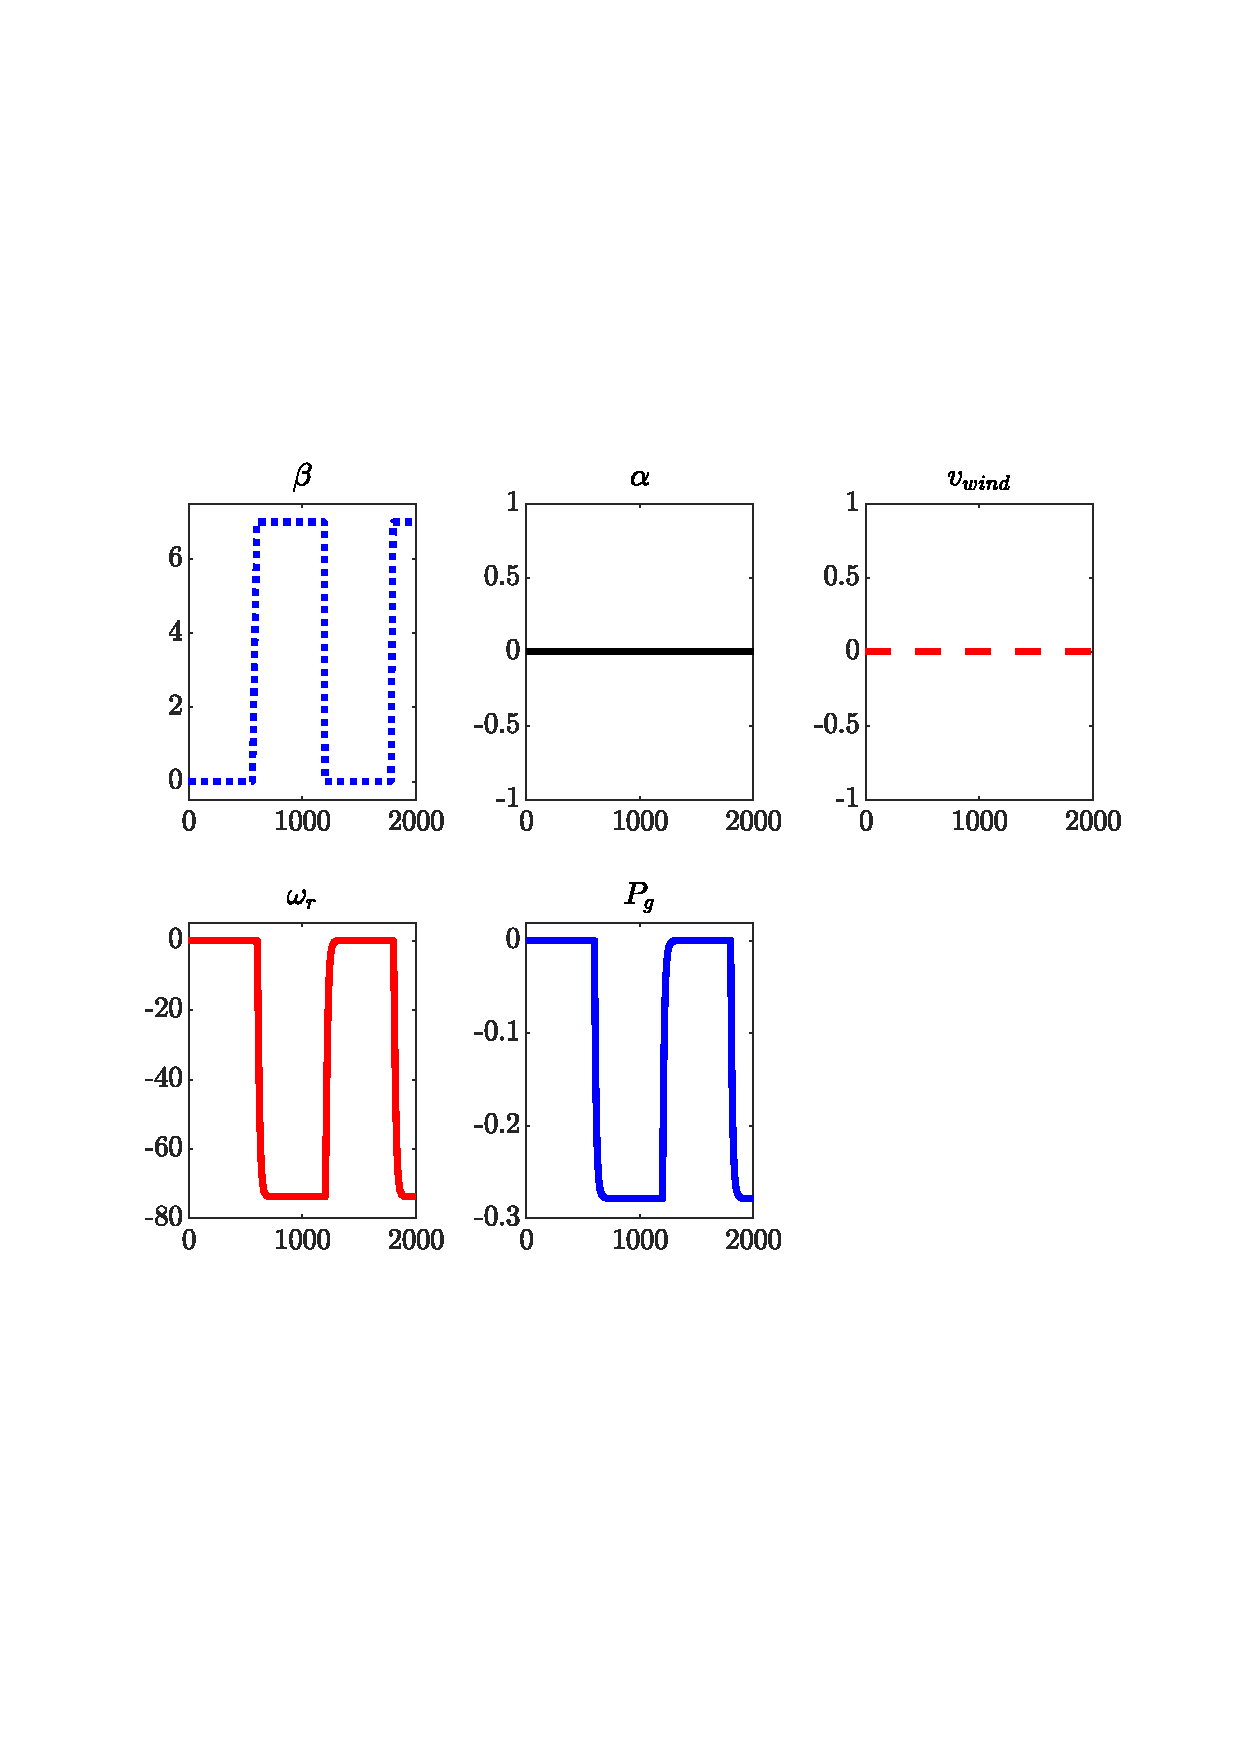
\includegraphics[scale=0.7,trim=60 200 50 150,clip]{fig/recreate_step_changes.pdf}
    \caption{Recreating subfigure $g_{11}$ by plotting inputs, outputs and the disturbance over time. A pulse with a period of \SI{1200}{\second} and a pulse width of \SI{600}{\second} changes $\beta$ by \SI{7}{\degree}. This results in reducing the rotational speed $\omega_r$ by \SI{70}{rpm}.}
    \label{fig:analysis:recreate_step_changes}
\end{figure}



\subsection{Relative Gain Array}  \label{sec:analysis:RGA}

The relative gain array is used to obtain a measure of the dependencies of inputs and outputs for a MIMO-system.
In this particular example we want to know the influence of rotational speed $\omega_r$ and the electrical power $P_g$ on pitch angle $\beta$ and duty cycle $\alpha$.


The RGA-matrix is symmetric and all column- and row-sums a equal to one.
For a $2\times2$-matrix we only need to calculate the element $(1,1)$ and deduce all other values.
\begin{align}
    \Lambda_{RGA} &= \begin{pmatrix}
        \lambda_{11} & \lambda_{12} \\
        \lambda_{21} & \lambda_{22}
    \end{pmatrix}, \text{with} \\
    & \lambda_{12} = \lambda_{21} \\
    & \lambda_{11} + \lambda_{12} = 1 \\
    & \lambda_{21} + \lambda_{22} = 1
\end{align}


\subsubsection*{Implementation in Matlab}


\begin{lstlisting}[style=Matlab-editor,caption={This Matlab function calculates a $2\times2$-RGA-matrix},captionpos=b,label={list:analysis:RGA}]
    function RGA = calculate_RGA(G_S_numerator)
        % Computation of RGA
        lambda_11 = G_S_numerator{1,1}/(G_S_numerator{1,1} - (G_S_numerator{1,2}*G_S_numerator{2,1})/G_S_numerator{2,2} );
        RGA = [[lambda_11, 1-lambda_11];[1-lambda_11,lambda_11]];
    end
\end{lstlisting}
    
In line four the RGA-matrix is calculated.
As previously described we only need to calculate  $\lambda_{11}$ and can deduce all other elements of $\Lambda$.

    

\subsubsection*{Results of RGA}

The investigation of the RGA for different wind speeds provides clearly different dependencies between the inputs and states.
The results are shown in \autoref{fig:analysis:RGA_results}.

\begin{figure}[H]
    \center
    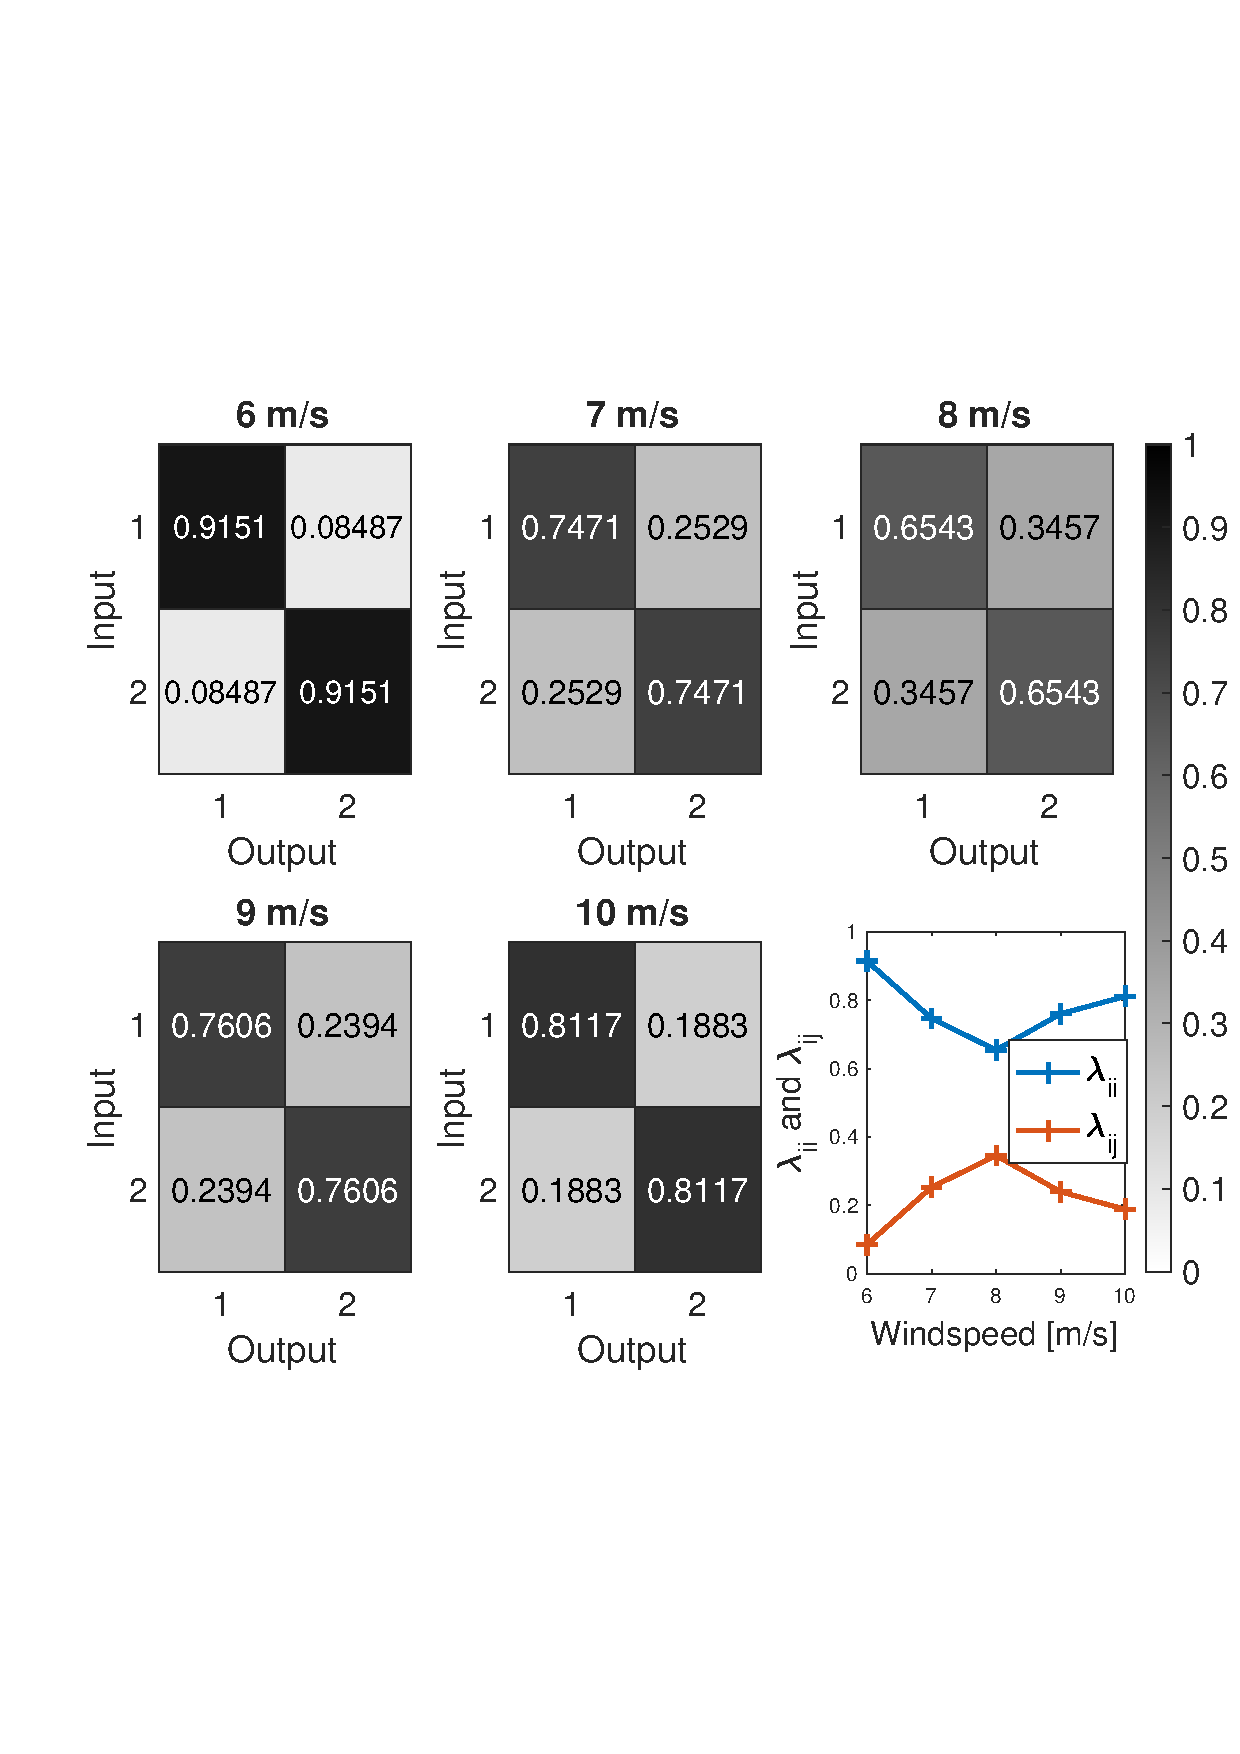
\includegraphics[scale=0.6,trim=40 180 0 120,clip]{fig/RGA_results.pdf}
    \caption{Visualization of the five RGA-matrices and a line plot for $\lambda_{ii}$ and $\lambda_{ij}$.}
    \label{fig:analysis:RGA_results}
\end{figure}

For very low windspeeds ($\SI{6}{\metre\per\second}$) the system is nearly decoupled.
At a windspeed of $\SI{10}{\metre\per\second}$, the system can also be considered almost decoupled.
If the the windspeed is approaching $\SI{8}{\metre\per\second}$ the peak coupling is reached.
This behaviour can be best seen at the line plot.
Both lines almost touch at a windspeed of $\SI{8}{\metre\per\second}$ and diverge before and after.

The results achieved are congruent with the findings of Fragaso et al. (\cite[p. 7]{Fragoso_et_al_2017}, \cite[p. 123]{Fragoso_PhD_2016})

In the following chapter we will design a controller for the \textit{hardest} condition of a coupled system with windspeeds of $\SI{8}{\metre\per\second}$.
